\documentclass[]{report}
\usepackage{amssymb,amsmath}
\usepackage{amsthm}
\usepackage{listings}
\usepackage[]{algorithm2e}
\usepackage[utf8]{inputenc}
\usepackage[francais]{babel}
\usepackage{graphicx}
\usepackage[unicode=true,
	colorlinks=false,
linkcolor=blue]{hyperref}

\hypersetup{breaklinks=true, pdfborder={0 0 0}}
\setlength{\parindent}{0pt}
\setlength{\parskip}{6pt plus 2pt minus 1pt}
\setlength{\emergencystretch}{3em}  % prevent overfull lines
\setcounter{secnumdepth}{0}

\title{Rapport du projet Starlight}
\author{Florian Knop (39310) - Gatien Bovyn (39189)}

\begin{document}
\lstset{language=C++}  
\maketitle

\newpage

\tableofcontents

\newpage

\section{Introduction}


Ce document vise à présenter le travail d’analyse et de programmation
effectué
lors de la réalisation du projet du laboratoire Langage C++~:~Starlight.

Ce projet a été réalisé en binôme par Florian Knop, matricule 39310 groupe 2G13,
et Gatien Bovyn, matricule 39189 groupe 2G11.

Le programme à concevoir consiste en une implémentation du modèle et d’une interface
graphique du jeu baptisé Starlight, puzzle à 2 dimensions basé sur la lumière.

Ce projet a été compilé principalement avec g++
(version 4.8.2 ou supérieure)
sous la distribution GNU/Linux Ubuntu (ou une de ses dérivées).
La version du framework Qt utilisée est la 5.0.2 ou supérieure.
Ce projet a été fait sous QtCreator, IDE OpenSource en version 2.8.1 ou
supérieure.

\section{Conventions}

\subsection{Conventions de nommage utilisées}

Dans cette section, nous présenterons les différentes conventions 
utilisées lors de ce projet. Nous avons décidé de reprendre certaines
conventions utilisées par la STL (Librairie Standard)
tout en utilisant d'autres conventions.

De manière globale, tous les noms de variables, classes, fichiers, etc.
sont en anglais.

\subsubsection{Fichiers}

Les noms de fichiers sont entièrement en minuscules
et possèdent les extensions \texttt{.h}
pour les headers et \texttt{.cpp} pour les fichiers sources.

\begin{itemize}
	\item \texttt{nomfichier.h}
	\item \texttt{nomfichier.cpp}
\end{itemize}

\subsubsection{Classes}

Les noms des classes commencent par une majuscule à chaque mot.
Cette convention est également valable pour les noms 
d'énumérations et structures.

\begin{itemize}
	\item \texttt{Classe}
	\item \texttt{NomClasse}
	\item \texttt{NomStruct}
	\item \texttt{NomEnumeration}
\end{itemize}

\newpage

\subsubsection{Variables}

\paragraph{Variables de classe}

Les noms des variables de classes sont en minuscules, les mots sont 
séparés par un underscore et le nom est suffixé par un underscore.

\begin{itemize}
	\item \texttt{variable\_}
	\item \texttt{nom\_variable\_}
\end{itemize}

Cette convention est également valable pour les variables d'une
structure.

\paragraph{Variables locales}

Les noms des variables locales respectent les mêmes conventions 
que les variables de classe, à la seule exception qu'ils ne sont pas
suffixés par un underscore.

\begin{itemize}
	\item \texttt{variable}
	\item \texttt{nom\_variable}
\end{itemize}

\paragraph{Constantes}

Les noms des constantes sont entièrement en majuscules et les mots sont
séparés par des underscores.

\begin{itemize}
	\item \texttt{CONSTANTE}
	\item \texttt{NOM\_CONSTANTE}
\end{itemize}

\subsubsection{Méthodes}

D'une manière générale, les noms de méthodes sont en minuscules et
séparés par des underscores.

\paragraph{Getters}

Le nom d'un getter (accesseur en lecture de variable de classe/structure)
est égal au nom de la variable de classe sans l'underscore final.

\begin{itemize}
	\item Variable : \texttt{variable\_} ~~-- Getter : \texttt{variable()}
	\item Variable : \texttt{nom\_var\_} ~~~~-- Getter : \texttt{nom\_var()}
\end{itemize}

\paragraph{Setters}

Le nom d'un setter (accesseur en écriture de variable de classe/structure)
est égal au nom de la variable sans l'underscore final préfixé de \texttt{set}.

\begin{itemize}
	\item Variable : \texttt{variable\_} ~~-- Setter : \texttt{set\_nom\_var()}
\end{itemize}

\paragraph{Autres méthodes}

Les autres méthodes possèdent les mêmes conventions que celles
énoncées ci-dessus.

\begin{itemize}
	\item \texttt{methode()}
	\item \texttt{nom\_methode()}
\end{itemize}

\subsubsection{Éléments d'une énumération} 

Les éléments d'une énumération suivent les mêmes conventions que celles des constantes énoncées ci-dessus.

\subsection{Autres conventions}

\newpage
\section{Présentation générale du projet}

Cette section décrit les objectifs principaux et secondaires effectués lors
de la réalisation de ce projet.
Toutes les classes utilisées sont décrites dans la section suivante.

Le projet fini ouvre sur un menu principal permettant
de jouer à Starlight, de voir les règles du jeu, d'accéder à l'éditeur de 
carte ou de simplement quitter.

\subsection{Le jeu}

Le projet permet de jouer à Starlight en important sa propre carte de jeu
au format \texttt{.lvl} qu'il est possible de créer soi-même grâce à l'éditeur
de carte (cf. \hyperref[Editeur]{«~Éditeur de cartes~»}).

Il est nécessaire de préciser que le jeu part du principe que la carte 
fournie est sans erreur. Une carte fournie avec erreur produira donc
un arrêt immédiat de l'application.

\subsubsection{Le fonctionnement du jeu}

Le but du jeu est de déplacer un rayon provenant d'une source lumineuse
pouvant être allumée ou éteinte
vers une destination à l'aide de miroirs plans amovibles réfléchissant
la lumière.
La lumière possède une longueur d'onde comprise dans le spectre
de lumière visible.

En addition avec leur déplacement, les miroirs peuvent tourner
autour d'un point de pivot.
Ce déplacement et cette rotation se font tout en restant
dans certaines limites si celles-ci ont été définies à la création du miroir.

Une gestion des collisions a également été implémentée pour
éviter que les miroirs déplacés ne heurtent les autres éléments de la carte.
De ce fait, la carte de jeu fournie par Mr. Absil a légèrement été modifiée
pour éviter que les miroirs ne se trouvent dans les murs à la création du niveau
et qu'il soit donc impossible de les déplacer par la suite.

La carte peut aussi posséder des cristaux qui modifient la longueur d'onde
du rayon les traversant, ainsi que des lentilles laissant passer la lumière
d'une certain intervalle de longueur d'onde.
La couleur de la lumière est donc modifiée selon la longueur d'onde 
du rayon lumineux.

Et pour finir, la carte peut être munie de bombes qui terminent et font perdre
instantanément la partie si celles-ci sont touchées par un rayon lumineux. 


\subsubsection{L'interface}

L'interface graphique du jeu Starlight a été réalisée sous Qt (en version 5.0.2 ou supérieure).
Il s'agit ici d'une interface simple et minimaliste permettant d'effectuer la fonction de base 
demandée : jouer.

La fenêtre de jeu possède également des menus permettant de :

\begin{itemize}
    \item \texttt{Quitter}
    \item \texttt{Revenir au menu principal}
    \item \texttt{Charger une carte}
    \item \texttt{Quitter la carte}
    \item \texttt{Voir les règles du jeu}
\end{itemize}

Les raccourcis clavier permettant d'accéder aux fonctions citées ci-dessus sont dépendants
du système d'exploitation utilisé.

Les miroirs sont sélectionnés en utilisant un double clic gauche.
Si un troisième clic s’ensuit, les limites de déplacement du pivot s'affichent
sous la forme d'un rectangle bleu.

Les miroirs peuvent être déplacés et tournés au clavier en utilisant les touches~:

\begin{itemize}
	\item \texttt{Z} pour déplacer vers le haut
	\item \texttt{S} pour déplacer vers le bas
	\item \texttt{Q} pour déplacer vers la gauche
	\item \texttt{D} pour déplacer vers la droite
	\item \texttt{Flèche directionnelle gauche} pour tourner dans le sens
		anti-horloger
	\item \texttt{Flèche directionnelle droite} pour tourner dans le sens
		horloger
    \item \texttt{Shift} + une des touches citées ci-dessus pour se déplacer / tourner
        plus vite
\end{itemize}

Des sons ont été ajoutés lorsque la source est allumée ou éteinte, 
lorsqu'une bombe a été touchée et lorsque la destination
est atteinte.

\paragraph{Faiblesses de l'interface} 

L'interface ne permet pas de déplacer les miroirs à la souris, mais seulement au clavier.
Le rectangle bleu affichant les limites du miroir s'affiche après un 3e clic plutôt 
que lors de la sélection du miroir.

Les sons ajoutés qui ont été cités ci-dessus ne s'activent pas toujours.
Par exemple lorsque la source est allumée et éteinte très vite.
Il se peut également que la source n'émette simplement pas de son.

\newpage
\subsection{\label{Editeur}Éditeur de cartes}

L’éditeur de carte a été conçu sur base du modèle et des vues existants.
Il reprend tous les éléments disponibles dans un niveau du jeu Starlight.

\subsubsection{Possibilités de l'éditeur}

Au lancement de l'éditeur, il est possible de charger un niveau existant 
ou d’en créer un nouveau en personnalisant sa taille. Celle-ci ne peut 
être changée par la suite.

Une fois chargé/créé, il est alors possible d’ajouter de nouveaux éléments 
dans le niveau (mur, miroir, lentille, cristal, bombe). Comme prévu par l'énoncé,
une seule source et une seule destination peuvent être incluses. Dès lors, 
celles-ci sont créées en même temps que le niveau et il n’est pas possible de 
les supprimer. Il n'est également pas possible de supprimer les murs extérieurs
au niveau.

Tous les éléments ont la possibilité d’être modifiés à tous niveaux, les setters
appropriés ayant été ajoutés dans les classes du modèle. Il est au minimum possible de déplacer
tous les éléments, soit par le panel droit qui offre la possibilité de modifier
un objet, soit par l'utilisation du clavier (Z pour le monter, S pour descendre, Q pour le translater
sur la gauche et D pour une translation vers la droite).

Une fois le niveau adapté, il est possible de le sauvegarder au format \texttt{.lvl}. 
La classe \texttt{MapWriter} a été écrite pour l'occasion, qui permet de sauver 
dans un fichier un niveau, comme \texttt{MapReader} permet de le lire.

Certaines options ont été désactivées dans l'éditeur pour rendre l'édition plus agréable,
notamment la gestion des collisions, les bruits et autres événements spéciaux.

\subsubsection{Faiblesses de l'éditeur}

La gestion des erreurs est totalement absente, ce qui signifie que l'utilisateur est 
responsable des données qu'il entre. Il est tout à fait possible de créer des éléments
dont les caractéristiques ne permettront pas de jouer une partie (une source en dehors
des limites par exemple).

La gestion dynamique des déplacements ne se fait que dans un sens, si l'on déplace un objet
à l'aide du clavier ses propriétés dans le panel de droite seront automatiquement modifiées.
Cependant, il faudra utiliser le bouton «~Appliquer~» du panel de droite afin que les changements
effectués à cet endroit entrent en application.

\newpage
\section{Présentation des différentes classes}

Dans cette section, nous allons décrire les différentes classes
composant ce projet.
L'implémentation du projet est divisée entre la partie modèle et la partie vue ainsi 
qu'une partie classes utilitaires.
Elle est également basée sur le design pattern «~Observateur~/~Observé~» comme demandé
dans les consignes. 

\subsection{\label{OO}Observateur / Observé}

Le design pattern Observateur / Observé a été implémenté à l'aide de deux classes : 

\begin{itemize}
    \item \texttt{ObserverInterface} qui représente l'observateur.
    \item \texttt{Observable} qui représente l'observé.
\end{itemize}

Pour plus d'informations sur les classes observées et observatrices, se référer à
\hyperref[AnnexeB]{«~l'Annexe B~»} de ce document.

\subsubsection{ObserverInterface}

La classe \texttt{ObserverInterface} est suffixée par \texttt{Interface} puisqu'il
s'agit d'une interface (pas au sens C++ car celui-ci ne possède pas la notion
d'interface) car cette classe ne possède que des méthodes \texttt{virtual} pures
qui sont donc obligées d'être redéfinies dans une classe héritant de celle-ci.
Cela définit donc parfaitement la notion d'interface.

Cette classe possède une méthode \texttt{notify(\dots)} qui est appelée à chaque fois
qu'une classe observée lance une notification (cf. \hyperref[Observable]{«~Observable~»}).

\subsubsection{\label{Observable}Observable}

La classe \texttt{Observable} représente l'observé. Celle-ci possède
une liste (\texttt{vector}) d'observateurs.
Un observé peut ajouter des observateurs à sa liste ou en supprimer grâces aux méthodes :
\begin{lstlisting}
    add_observer(ObserverInterface * obs);
    remove_observer(ObserverInterface * obs);
\end{lstlisting}

Un observé peut lancer des notifications via la méthode :
\begin{lstlisting}
notify_all(Observable * obs, 
            std::string& msg, 
            std::vector<std::string>& args = std::vector<string>())
\end{lstlisting}

Cette méthode appellera pour chaque observateur la méthode \texttt{notify(\dots)} de ce dernier.
Nous avons choisi de créer 3 paramètres pour les notifications, dont une liste d'arguments optionnelle.

Dans un premier temps, la notification envoie un pointeur vers l'observé, cela peut être utile si l'observateur
ne peut pas savoir qui a envoyé une notification, grâce à ce pointeur, il peut donc agir sur l'objet. De plus, un message
de notification est envoyé, cela sert à effectuer différentes tâches selon le message envoyé.

Et pour finir, une liste d'arguments est également envoyée. Cette dernière nous a servi principalement pour la gestion
de collisions où il a fallu envoyer le déplacement voulu en paramètre pour que le niveau puisse vérifier si ce déplacement est
possible pour ensuite réagir en conséquence.

\subsection{Les classes/namespaces utilitaires}

\subsubsection{MapReader}

La classe \texttt{MapReader} est la classe qui lit un fichier \texttt{.lvl} 
et crée le niveau (cf. \hyperref[Level]{«~Level~»}).

Cette classe considère que le fichier est sans erreur. Une instantiation d'objets
erronés produira donc un arrêt de l'application.

Cette classe est basée sur le \texttt{Singleton Pattern}. On ne peut qu’instancier un niveau
à la fois.

\subsubsection{MapWriter}

La classe \texttt{MapWriter} est la classe qui va écrire un niveau (cf. \hyperref[Level]{«~Level~»}) 
dans un fichier texte. Il s’agit donc du processus inverse de la classe
\texttt{MapReader}. Cette classe sert à l’éditeur lors de la sauvegarde de la
carte en cours d’édition.

\subsubsection{\label{Constants}Constants}

\texttt{constants.h} est un header reprenant toutes les constantes utilisées
dans ce projet. 

\begin{itemize}
    \item \texttt{INF} correspond à l'infini.
    \item \texttt{EPSILON} correspond à \texttt{0.00001}. EPSILON permet
        d'éviter les imprécisions entre deux nombres réels (cf. \hyperref[equals]{«~umath - méthode equals()~»}).
    \item \texttt{PI} correspond à la valeur de PI \texttt{3.14159\dots} avec
        autant de décimales possibles qu'un \texttt{double} peut contenir.
    \item \texttt{PI\_2} correspond à la valeur de PI divisé par deux.
    \item \texttt{PI\_4} correspond à la valeur de PI divisé par quatre.
    \item \texttt{PI\_2\_3} correspond à la valeur de PI\_2 multiplié par trois.
\end{itemize}

\subsubsection{Le namespace umath}

Le namespace \texttt{umath} possède toutes les méthodes utilitaires mathématiques
et géométriques servant au projet. Comme par exemple des méthodes permettant de trouver
les intersections entre droites, segments, ellipses et rectangles.

\label{equals}
\texttt{umath} reprend des méthodes d'égalité de nombre réels. Deux nombres réels sont égaux
si la valeur absolue de la soustraction de ceux-ci est plus petite que la valeur de EPSILON (cf. \hyperref[Constants]{«~Constants~»}).


Une autre méthode d’égalité permet de vérifier si un nombre équivaut à l’infini (INF ou -INF).
Il y a également des méthodes de conversions entre pentes, radians, degrés, etc.

Les méthodes d’intersections sont décrites plus en détails dans la section \hyperref[Annexe]{Annexe - Démarches mathématiques}.

\subsection{Modèle}

Dans cette section, nous allons décrire les différentes classes du modèle 
(classes métiers).
Un squelette de classes a été fourni par Monsieur Absil.
Ce squelette contenait les fichiers suivants~:
\texttt{point.h}, \texttt{source.h}, \texttt{dest.h}, \texttt{nuke.h}, \texttt{wall.h},
\texttt{crystal.h}, \texttt{lens.h}, \texttt{mirror.h}, \texttt{ray.h}, \texttt{level.h} ainsi que leurs sources correspondantes.
Nous avons décidé de modifier ce squelette tout en gardant la 
structure générale.

\subsubsection{\label{Point}Point}

La classe \texttt{Point} représente une position dans un espace à deux dimensions. 
Elle est munie des coordonnées \texttt{x} et \texttt{y} qui sont tous deux des
nombres réels (\texttt{double}). 

La classe \texttt{Point} fourni par Mr. Absil comprenait des coordonnées entières.
Nous avons décidé de passer les coordonnées en nombres réels par souci de précision.

La classe permet également de calculer la distance entre deux points grâce à la formule~:

$$ \sqrt[2]{(x_1 - x_2)^2 + (y_1 - y_2)^2} $$

\newpage
\subsubsection{\label{Line}Line}

La classe \texttt{Line} représente une droite de la forme~: 
$ D \equiv ax + by + c = 0 $ \\

$ D \equiv ax + c = 0 $ représente l'équation d'une droite verticale (b = 0). \\
$ D \equiv by + c = 0 $ représente l'équation d'une droite horizontale (a = 0). \\

Elle possède les trois paramètres $ a $, $ b $ et $ c $ ainsi que l'angle
que forme la droite pour éviter de devoir reconvertir la pente calculée par $ \frac{-a}{b} $
en angle à chaque fois.

La classe \texttt{Line} possède des méthodes permettant de savoir si celle-ci est 
verticale ($ b = 0 $) ou horizontale ($ a = 0 $), si elle est perpendiculaire ou parallèle à une autre droite.
Des méthodes permettant d'obtenir $ x $ selon une valeur de $ y $ donné et
inversement sont également
présentes. Cependant ces méthodes peuvent renvoyer une valeur infinie dans le cas où la droite 
est soit verticale, soit horizontale.

Cette classe sert principalement à modéliser un rayon de lumière (cf. \hyperref[Ray]{«~Ray~»}) pour trouver 
les intersections\footnote{\hyperref[AnnexeIntersects]{«~Annexe A - Démarche mathématique : Intersections~»}} entre le rayon et les éléments du jeu.

\subsubsection{\label{LineSegment}LineSegment}

La classe \texttt{LineSegment} représente un segment de droite possédant
deux points (cf. \hyperref[Point]{«~Point~»}) qui sont les extrémités du segment.

Nous avons fait le choix qu'un segment puisse posséder deux fois le même point.
Bien que cela n'ait pas vraiment de sens purement mathématique, un segment
ayant deux fois le même point est tout simplement un point.

Le segment peut être transformé en droite grâce aux deux points
le constituant et ainsi former l'équation de droite.

Le segment peut également être décalé d'un certain $ x $ et $ y $ ainsi que tourné 
d'un certain angle\footnote{\hyperref[AnnexeRotation]{«~Annexe A - Démarche mathématique : Rotation de segment~»}}.

\subsubsection{\label{Ellipse}Ellipse}

La classe \texttt{Ellipse} représente une forme géométrique de type elliptique.
Elle possède un point central ainsi qu'un rayon $x$ et $y$. Si ces deux
rayons sont égaux, il s'agit alors d'un cercle.

Cette classe sert à représenter les objets \texttt{Lens} (cf. \hyperref[Lens]{«~Lens~»}) et \texttt{Crystal} (cf. \hyperref[Crystal]{«~Crystal~»}).

\subsubsection{\label{Rectangle}Rectangle}

La classe \texttt{Rectangle} représente une forme géométrique rectangulaire.
Elle possède un point supérieur gauche ainsi qu'une longueur et hauteur 
nous permettant de retrouver facilement les autres extrémités de la 
forme.

Cette classe sert à représenter les objets \texttt{Source} (cf. \hyperref[Source]{«~Source~»}) et \texttt{Dest} (cf. \hyperref[Dest]{«~Dest~»}).

\subsubsection{\label{Element}Element}

La classe \texttt{Element} est la super-classe de tous les éléments pouvant
se trouver sur une carte de jeu.
Il s'agit de :

\begin{itemize}
    \item \texttt{Source}
    \item \texttt{Dest}
    \item \texttt{Wall}
    \item \texttt{Mirror}
    \item \texttt{Lens}
    \item \texttt{Crystal}
    \item \texttt{Nuke}
\end{itemize}

La classe \texttt{Ray} (cf. \hyperref[Ray]{«~Ray~»}) n’est pas un élément, les éléments concernent 
les objets pouvant interagir avec un rayon.
Il s'agit principalement d'une classe \texttt{tag} pouvant
donner le type de l'élément. Son rôle est de pouvoir retrouver
le type d'un objet lors d'une intersection (cf. \hyperref[Level]{«~Level~»}).

Une énumération fortement typée est donc présente. Elle s'appelle
\texttt{Type} et reprend les noms des éléments cités ci-dessus.

\texttt{Element} hérite de l'interface \texttt{Observable} (cf. \hyperref[OO]{«~Observable/Observer~»}) et chaque
sous-classe est observée par la vue correspondante.
    
\subsubsection{\label{Source}Source}

La classe \texttt{Source} représente la source lumineuse du jeu.
Elle est de forme rectangulaire et peut donc être transformée
en \texttt{Rectangle} (cf. \hyperref[Rectangle]{«~Rectangle~»}).

Le rayon lumineux part du coin supérieur gauche de la source et possède
un angle par rapport à l'axe des abscisses. Il possède aussi une longueur
d'onde de départ.

\paragraph{Dans l'interface} cf. \hyperref[SourceView]{«~SourceView~»}.

\subsubsection{\label{Dest}Dest}

La classe \texttt{Dest} représente la destination à atteindre par 
le rayon lumineux. Elle est de forme rectangulaire comme la source
et peut également être transformée en \texttt{Rectangle} (cf. \hyperref[Rectangle]{«~Rectangle~»}).

\paragraph{Dans l'interface} cf. \hyperref[DestinationView]{«~DestinationView~»}

\subsubsection{\label{Wall}Wall}

La classe \texttt{Wall} représente un mur du jeu qui bloque les rayons
lumineux. Un mur est un segment de droite et peut donc être transformé 
en segment de droite (cf. \hyperref[LineSegment]{«~LineSegment~»}).

\paragraph{Dans l'interface} cf. \hyperref[WallView]{«~WallView~»}

\subsubsection{\label{Mirror}Mirror}

La classe \texttt{Mirror} représente un miroir. Un miroir
est un segment de droite qui réfléchit la lumière.
Un miroir peut donc être transformé en 
segment de droite (cf. \hyperref[LineSegment]{«~LineSegment~»}).

\paragraph{Dans l'interface} cf. \hyperref[MirrorView]{«~MirrorView~»}

\subsubsection{\label{Lens}Lens}

La classe \texttt{Lens} représente une lentille. Une lentille est
une ellipse possédant un intervalle de longueur d'onde. Le rayon doit
être dans cet intervalle pour pouvoir traverser la lentille, dans le cas
contraire, elle agira comme un mur.

Étant de forme elliptique, la lentille peut être transformée en Ellipse (cf. \hyperref[Ellipse]{«~Ellipse~»}).

\paragraph{Dans l'interface} cf. \hyperref[LensView]{«~LensView~»}

\newpage
\subsubsection{\label{Crystal}Crystal}

La classe \texttt{Crystal} représente un cristal. Un cristal est un cercle
possédant un modificateur de longueur d'onde. Quand un rayon le traverse, ce dernier
en ressort avec une longueur d'onde différente. 

Comme un cercle est également une ellipse, celui-ci peut également être transformé en Ellipse (cf. \hyperref[Ellipse]{«~Ellipse~»}).

\paragraph{Dans l'interface} cf. \hyperref[CrystalView]{«~CrystalView~»}

\subsubsection{\label{Nuke}Nuke}

La classe \texttt{Nuke} représente une bombe de forme circulaire.
Quand un rayon croise une bombe, la partie est instantanément terminée et perdue. Cela est accompagnée
d'un message de fin de partie.

Comme un cercle est également une ellipse, celui-ci peut également être transformé en Ellipse (cf. \hyperref[Ellipse]{«~Ellipse~»}).

\paragraph{Dans l'interface} cf. \hyperref[NukeView]{«~NukeView~»}

\subsubsection{\label{Ray}Ray}

La classe \texttt{Ray} représente un rayon. Un rayon est un segment de droite reliant
deux objets de la carte. 

Un rayon est dans un premier temps (avant sa création) transformé en \texttt{Line} (cf. \hyperref[Line]{«~Line~»}) pour
trouver les intersections\footnote{\hyperref[AnnexeIntersects]{«~Annexe A - Démarche mathématique : Intersections~»}} entre le rayon et les objets de la cartes. Une fois la bonne intersection trouvée (le point final du rayon), le rayon peut être créé et 
transformé en \texttt{LineSegment} (cf. \hyperref[LineSegment]{«~LineSegment~»}) à l'affichage.

\paragraph{Dans l'interface} cf. \hyperref[RayView]{«~RayView~»}

\newpage
\subsubsection{\label{Level}Level}

La classe \texttt{Level} est de loin la classe la plus importante du modèle.
Il s'agit de la classe représentant un niveau, elle gère toute la logique métier
du jeu. C'est elle qui contient tous les éléments du jeu et qui calcule
la trajectoire du rayon lumineux.

\paragraph{Explications} : la logique métier \\

La logique métier est composée de méthodes principales : 

\begin{lstlisting}
void compute_rays();
void compute_ray(const Line& line, const Point& start, int wl);
void get_intersections(const Line& line, const Point& start);
\end{lstlisting}

\texttt{compute\_rays()} crée la première droite composant le rayon par rapport à l'angle de la 
source et son point de départ, il appelle ensuite \texttt{compute\_ray(\dots)} qui va chercher
l'intersection la plus proche en appelant \texttt{get\_intersections(\dots)}. Cette dernière méthode
va remplir un vecteur (\texttt{vector}) d'\texttt{Intersection} qui est une structure créée dans 
le header \texttt{level.h}. Cette structure reprend le point d'intersection ainsi que l'élément relié à ce point.

\texttt{get\_intersections(\dots)} va chercher des intersections avec la droite qu'il reçoit en paramètre
et tous les objets du jeu. Chaque intersection avec un objet sera alors mise dans le vecteur d'intersection
si cette intersection se trouve du bon côté du point \texttt{start} par rapport à l'angle du rayon.

Toutes les intersections seront ensuite triées dans l'ordre croissant selon la distance entre le point \texttt{start} et
l'intersection grâce à une expression lambda.
La première valeur du vecteur devrait alors correspondre à l'intersection la plus proche dans l'axe du rayon.

\texttt{compute\_ray(\dots)} va dans un premier temps créer le rayon entre le point \texttt{start} et le point d'intersection.
Par la suite, avec la première valeur du vecteur d'intersections, 
\texttt{compute\_ray(\dots)} va effectuer ce qu'il faut selon le type de l'élément déterminé 
grâce à la super-classe \texttt{Element} (cf. \hyperref[Element]{«~Element~»}).

Un booléen sera mis à vrai ou faux selon le cas. À la fin de la méthode, si ce booléen vaut donc vrai, cela veut dire
que le rayon peut continuer. Un appel récursif à \texttt{compute\_ray(\dots)} est donc fait avec les nouvelles valeurs. 

\paragraph{Dans l'interface} cf. \hyperref[MapView]{«~MapView~»}    

\subsection{Vue}

L'interface graphique a été réalisée en Qt à la main (sans l'aide de \texttt{QtDesigner}).
Chaque élément visuel dispose d’un pointeur vers son
équivalent dans le modèle, sur base duquel il est construit. Il observe également cet élément afin de se mettre
à jour automatiquement.

Chaque élément a également été prévu pour être utilisé dans l'éditeur, et dispose ainsi d’un booléen pour le rendre 
sélectionnable quand cela est nécessaire.

Les classes composant la partie vue de l'application sont~:

\subsubsection{ElementView}

Classe servant de super-classe à tous les éléments présents sur un \texttt{MapView}.
Il s'agit de :

\begin{itemize}
    \item \texttt{SourceView}
    \item \texttt{DestinationView}
    \item \texttt{WallView}
    \item \texttt{MirrorView}
    \item \texttt{LensView}
    \item \texttt{CrystalView}
    \item \texttt{NukeView}
\end{itemize}

\subsubsection{\label{SourceView}SourceView}

Classe représentant une source lumineuse sur le plateau de jeu. Bien que dans les consignes, la source lumineuse soit un carré, nous avons ensuite utilisé des images pour la représenter.
La source dispose de 2 états, allumée ou éteinte qui peut être changé grâce à un double clic.
Passer d’un état à l'autre change l'image la représentant et produit un son d’interrupteur.

Cette classe hérite de \texttt{QGraphicsPixmapItem} pour pouvoir représenter une image.
\texttt{SourceView} hérite également de l'interface \texttt{ObserverInterface} (cf. \hyperref[OO]{«~Observable/Observer~»}) et observe
la classe \texttt{Source} qu'elle modélise.

\subsubsection{\label{DestinationView}DestinationView}

La classe \texttt{DestinationView} modélise la destination à atteindre par le rayon émis depuis la source pour gagner la partie.
La destination devient verte une fois atteinte. De plus, un message de victoire est affiché.

Cette classe hérite de \texttt{QGraphicsRectItem} pour pouvoir représenter un rectangle.
\texttt{DestinationView} hérite également de l'interface \texttt{ObserverInterface} (cf. \hyperref[OO]{«~Observable/Observer~»}) et observe
la classe \texttt{Dest} qu'elle modélise.

\subsubsection{\label{WallView}WallView}

La classe \texttt{WallView} modélise un mur, élément visuel sur lequel le rayon est stoppé. 
Les murs sont représentés par des segments de droite noirs.

Cette classe hérite de \texttt{QGraphicsLineItem} pour pouvoir représenter un segment.
\texttt{WallView} hérite également de l'interface \texttt{ObserverInterface} (cf. \hyperref[OO]{«~Observable/Observer~»}) et observe
la classe \texttt{Wall} qu'elle modélise.

\subsubsection{\label{MirrorView}MirrorView}

La classe \texttt{MirrorView} modélise un miroir sur lequel un rayon peut être réfléchi.
Le miroir est représenté par un segment de droite rouge. Ce dernier, une fois sélectionné, affiche
un rectangle bleu affichant les limites de déplacement du pivot. 

Cette classe hérite de \texttt{QGraphicsLineItem} pour pouvoir représenter un segment.
\texttt{MirrorView} hérite également de l'interface \texttt{ObserverInterface} (cf. \hyperref[OO]{«~Observable/Observer~»}) et observe
la classe \texttt{Mirror} qu'elle modélise.

\subsubsection{\label{LensView}LensView}

La classe \texttt{LensView} modélise une lentille à travers laquelle un rayon peut passer si sa longueur d’onde est
comprise entre les valeurs de la lentille. Sinon la lentille se comporte comme un mur et le rayon 
est stoppé. 

Cette classe hérite de \texttt{QGraphicsEllipseItem} pour pouvoir représenter une ellipse.
\texttt{LensView} hérite également de l'interface \texttt{ObserverInterface} (cf. \hyperref[OO]{«~Observable/Observer~»}) et observe
la classe \texttt{Lens} qu'elle modélise.

\subsubsection{\label{CrystalView}CrystalView}

La classe \texttt{CrystalView} modélise un cristal, élément ovale qui modifie la longueur d’onde d’un rayon si
celui-ci traverse ledit cristal.

Cette classe hérite de \texttt{QGraphicsEllipseItem} pour pouvoir représenter une ellipse.
\texttt{CrystalView} hérite également de l'interface \texttt{ObserverInterface} (cf. \hyperref[OO]{«~Observable/Observer~»}) et observe
la classe \texttt{Crystal} qu'elle modélise.

\subsubsection{\label{NukeView}NukeView}

Classe représentant une bombe, élément explosif du plateau qui fait perdre la partie
si touché par un rayon lumineux (\texttt{RayView}). Dès le moment où elle est illuminée, une bombe
change de couleur (passe du noir au rouge) et produit un son et un message visuel indiquant la fin de partie.

Cette classe hérite de \texttt{QGraphicsEllipseItem} pour pouvoir représenter une ellipse.
\texttt{NukeView} hérite également de l'interface \texttt{ObserverInterface} (cf. \hyperref[OO]{«~Observable/Observer~»}) et observe
la classe \texttt{Nuke} qu'elle modélise.

\subsubsection{\label{RayView}RayView}

Classe modélisant un rayon lumineux, émis depuis la source (\texttt{SourceView}) et destiné à atteindre la destination 
(\texttt{DestView}) en se reflétant sur des miroirs et en passant à travers des cristaux si nécessaire.
Un \texttt{RayView} a une couleur différente selon sa longueur d’onde comme proposé dans les objectifs secondaires,
cette couleur reflétant la couleur réelle qu’aurait un rayon lumineux de cette longueur d’onde.

Cette classe hérite de \texttt{QGraphicsLineItem} pour pouvoir représenter un segment.

\subsubsection{\label{MapView}MapView}

Classe représentant le plateau de jeu, où tous les éléments sont disposés et affichés.
Elle s’occupe de gérer les raccourcis clavier utilisés pour déplacer/pivoter les
miroirs dans le jeu et de déplacer les éléments en général dans l'éditeur de carte.


\subsection{\label{EditeurClasses}L'éditeur de carte}

\subsubsection{\label{MainEditor}MainEditor}

Widget principal de l'éditeur de carte qui contient les classes qui suivent.
Il est composé de 3 widgets principaux~:~\texttt{Elements} qui représente le panel gauche, une \texttt{MapView} qui 
représente le niveau à modifier (widget central) et \texttt{Properties}, widget droit qui servira à modifier les 
caractéristiques des éléments de la carte.

\subsubsection{\label{Elements}Elements}

Widget de gauche de l'éditeur, permet de créer un nouveau niveau de hauteur et
largeur définies par l'utilisateur.
Permet également d’ajouter des éléments à la carte~:~miroir, bombe, cristal et lentille. La source et la destination étant uniques, 
elles sont directement ajoutées lors de la création d’un niveau.

\subsubsection{\label{Properties}Properties}

Widget de droite de l’éditeur, permet de modifier les caractéristiques des éléments présents dans la carte éditée.
L'édition est individuelle (il n’est pas possible de déplacer plusieurs éléments
en même temps par exemple) mais complète (chaque attribut de l'objet peut être modifié).

\subsubsection{\label{PropertiesInterface}PropertiesInterface}

Les classes héritant de PropertiesInterface :

\begin{itemize}
    \item \texttt{SourceProp}
    \item \texttt{DestProp}
    \item \texttt{WallProp}
    \item \texttt{MirrorProp}
    \item \texttt{LensProp}
    \item \texttt{CrystalProp}
    \item \texttt{NukeProp}
\end{itemize}

Super-classe abstraite, permet à \texttt{Properties} d’interagir avec n’importe quelle classe \texttt{*Prop} de manière transparente, 
notamment pour les boutons «~Apply~» et «~Reset~».
Les classes qui héritent de \texttt{PropertiesInterface} sont spécifiques à chaque élément du modèle 
(\texttt{Crystal}, \texttt{Dest}, \texttt{Lens}, \texttt{Mirror}, \texttt{Nuke}, \texttt{Source} et \texttt{Wall}).
Chaque élément héritant de \texttt{PropertiesInterface} hérite également de
\texttt{Observer}, ce qui permet de mettre à jour les propriétés dans le panel
si l'élément est bougé sur la \texttt{MapView} à l'aide du clavier.

\subsubsection{\label{CrystalProp}CrystalProp}

Widget composé de plusieurs spinbox permettant de modifier la position, le rayon et le modificateur de rayon
d'un cristal. Tous les spinbox vont de 0 à 999.

\subsubsection{\label{DestProp}DestProp}

Widget composé de plusieurs spinbox permettant de modifier la position et la longueur de la destination. Tous les spinbox vont de 0 à 999.

\subsubsection{\label{LensProp}LensProp}

Widget composé de plusieurs spinbox permettant de modifier la position, la hauteur, la largeur, 
la longueur d’onde minimale et la longueur d’onde maximale autorisées pour qu’un rayon passe à travers de la lentille.
Tous les spinbox vont de 0 à 999.

\subsubsection{\label{MirrorProp}MirrorProp}

Widget composé de plusieurs spinbox permettant de modifier la position, la longueur, la distance entre le pivot 
et l’extrémité gauche du miroir, l’angle d’inclinaison, les positions minimales et maximales que peut prendre le miroir, 
ainsi que les angles minimum et maximum autorisés pour le miroir. Tous les spinbox vont de 0 à 999.

\subsubsection{\label{NukeProp}NukeProp}

Widget composé de plusieurs spinbox permettant de modifier la position et le rayon d’une bombe. Tous les spinbox vont de 0 à 999.

\subsubsection{\label{SourceProp}SourceProp}

Widget composé de plusieurs spinbox permettant de modifier la position, la largeur du carré représentant la source, 
l’angle du rayon émis par la source et la longueur d’onde du dit rayon. Tous les spinbox vont de 0 à 999.

\subsubsection{\label{WallProp}WallProp}

Widget composé de plusieurs spinbox permettant de modifier la position des 2 extrémités d’un mur. Tous les spinbox vont de 0 à 999.

\section{Les bugs connus}

La méthode 
\begin{lstlisting}
umath::is_on_good_side(const Line& l, 
                       const Point& ref,
                       const Point& start);
\end{lstlisting}
peut avoir des problèmes de précision, ce qui fait que l'intersection, bien que du bon côté, ne sera pas 
prise en compte dans le vecteur d'intersections, ce qui résultera en un vecteur d'intersections vide. Et donc un
accès au premier élément sur un vecteur vide produira un \texttt{out\_of\_range} quittant l'application.

Pour éviter donc ce crash énoncé ci-dessus, nous avons fait en sorte que le rayon ne continue pas si le vecteur 
devient vide par erreur.


\section{Conclusion}

\section{Bibliographie}

Les sons utilisés ont été produits par Mike Koenig et sont sous licence Attribution 3.0.\\

\href{http://soundbible.com/106-Car-Explosion.html}{Bruit de bombe}   \\
\href{http://soundbible.com/1003-Ta-Da.html}{Bruit de victoire}       \\
\href{http://soundbible.com/761-Switch.html}{Bruit d’interrupteur}    \\

\section{\label{Annexe}Annexes}

\subsection{Annexe A : Démarches mathématiques}

\subsubsection{\label{AnnexeRotation}Rotation de segment}

La méthode de rotation de segment utilisée se base sur les formules
de coordonnées polaires\footnote{\href{http://fr.wikipedia.org/wiki/Coordonn\%C3\%A9es\_polaires}{Wikipedia : Coordonnées polaires}}
ainsi que les formules trigonométriques d'additions
\footnote{\href{http://fr.wikipedia.org/wiki/Trigonom\%C3\%A9trie}{Wikipedia : Formules trigonométriques}}.

Pour tourner un segment, il faut un point de pivot. Ce point de pivot
doit ensuite être déplacé sur l'origine du repère $ (0, 0) $.

Les formules de coordonnées polaires pour $ x $ et $ y $ sont :
$$ x = r \cdot \cos{q} $$ 
$$ y = r \cdot \sin{q} $$

$ r $ correspond à la distance entre l'origine et le point et $ q $ correspond 
à l'angle entre l'axe des abscisses et la droite formée avec l'origine et le point.

Lorsque l'on souhaite tourner un segment et trouver $ x' $ et $ y' $, 
il suffit d'augmenter ou diminuer l'angle $ q $ par un angle $ f $ comme ceci~:

$$ x' = r \cdot \cos{q + f} $$
$$ y' = r \cdot \sin{q + f} $$

Grâce aux formules trigonométriques d'additions, on peut transformer ce résultat en~:

$$ x' = r \cdot \cos{q} \cdot \cos{f} - r \cdot \sin{q} \cdot \sin{f} $$
$$ y' = r \cdot \sin{q} \cdot \cos{f} - r \cdot \cos{q} \cdot \sin{f} $$

Et pour finir, en remplaçant les deux premières égalités dans cette dernière on obtient~: 

$$ x' = x \cdot \cos{f} - y \cdot \sin{f} $$
$$ y' = x \cdot \sin{f} + y \cdot \cos{f} $$

Il faut ensuite redéplacer le pivot à son point de départ.

\newpage
\subsubsection{\label{AnnexeIntersects}Trouver l'intersection entre deux droites}

Une droite possède une intersection avec une autre droite si :
\begin{itemize}
    \item Celles-ci sont parallèles et confondues, alors l'intersection est la droite elle-même.
    \item Celles-ci sont non parallèles, alors l'intersection est un point. \\
\end{itemize} 

$ D \equiv ax + by + c = 0 $ représente l'équation d'une droite. \\
$ D \equiv ax + c = 0 $ représente l'équation d'une droite verticale ($b = 0$). \\
$ D \equiv by + c = 0 $ représente l'équation d'une droite horizontale ($a = 0$). \\

On commence donc dans un premier temps à tester si les deux droites sont parallèles. \\

Soit deux droites $D_1$ et $D_2$, ces deux droites sont parallèles si : 
$$ a_1 \cdot b_2 - a_2 \cdot b_1 = 0 $$

\begin{proof}
La pente d'une droite vaut $\frac{-a}{b}$ et deux droites sont parallèles
si leurs pentes sont égales. Il suffit donc de modifier l'équation en passant chaque terme du bon côté. \\
$ a_1 \cdot b_2 = a_2 \cdot b_1 $ puis ensuite : $ \frac{a_1}{b_1} = \frac{a_2}{b_2} $ ce qui équivaut à
$ \frac{-a_1}{b1} = \frac{-a_2}{b_2} $ \\
\end{proof}

Si les deux droites sont parallèles : 
\begin{itemize}
    \item Les deux droites sont verticales : si leurs $x$ sont égaux, elles sont confondues.
    \item Les deux droites sont horizontales : si leurs $y$ sont égaux, elles sont confondues.
    \item Les droites ne sont ni verticales, ni horizontales, il faut alors tester si les deux
        ordonnées à l'origine sont égales. Cette dernière vaut $\frac{-c}{b}$. \\
\end{itemize}

Si les deux droites ne sont pas parallèles, il faut remplacer une variable de $D_1$ dans $D_2$
ou inversement pour trouver la deuxième variable. On a choisi de remplacer $y$.
On a donc l'égalité suivante : 

$$ x = \frac{(c_1 \cdot b_2 - c_2 \cdot b_1)}{(a_2 \cdot b_1 - a_1 \cdot b_2)} $$

\begin{proof}
$$ D_1 \equiv y = \frac{-a_1 \cdot x}{b_1} - \frac{c_1}{b_1} $$
$$ D_2 \equiv y = \frac{-a_2 \cdot x}{b_2} - \frac{c_2}{b_2} $$

On remplace $y$ de $D_1$ dans $D_2$ :

$$ \frac{-a_1 \cdot x}{b_1} - \frac{c_1}{b_1} = \frac{-a_2 \cdot x}{b_2} - \frac{c_2}{b_2} $$

Il ne reste plus qu'à simplifier :

$$ \frac{-a_1 \cdot x}{b_1} + \frac{a_2 \cdot x}{b_2} = \frac{c_1}{b_1} - \frac{c_2}{b_2} $$
$$ \frac{(-a_1 \cdot x \cdot b_2) + (a_2 \cdot x \cdot b_1)}{(b_1 \cdot b_2)} = \frac{(c_1 \cdot b_2 - c_2 \cdot b_1)}{(b_1 \cdot b_2)} $$
$$ (a_2 \cdot b_1 \cdot x) - (a_1 \cdot b_2 \cdot x) = (c_1 \cdot b_2 - c_2 \cdot b_1) $$
$$ x \cdot ((a_2 \cdot b_1) - (a_1 \cdot b_2)) = (c_1 \cdot b_2 - c_2 \cdot b_1) $$
$$ x = \frac{(c_1 \cdot b_2 - c_2 \cdot b_1)}{(a_2 \cdot b_1 - a_1 \cdot b_2)} $$ \\
\end{proof}

Maintenant que nous avons la coordonnée $x$, il suffit de la remplacer
dans une des deux équations $D_1$ ou $D_2$ pour trouver le $y$ 
correspondant.

\subsubsection{Trouver l'intersection entre une droite et un segment de droite}

L'intersection entre une droite et un segment ressemble très fort
à l'intersection entre deux droites tout simplement car il faudra transformer
le segment en droite pour trouver une intersection entre ces deux droites
puis ensuite de vérifier si cette intersection se trouve bien dans le domaine
$x$ et $y$ du segment.

La différence est que l'intersection peut être un segment entier si la droite
et le segment sont confondus.

Pour transformer un segment en droite : \\
Soit $A$ et $B$ les deux extrémités du segment, les paramètres de la droite valent : 
$ a = A.y - B.y $ \\
$ b = B.x - A.x $ \\
$ c = (A.x \cdot B.y) - (A.y \cdot B.x) $ \\

\subsubsection{Trouver l'intersection entre deux segments}

Dans le cas de l'intersection segment/segment, il faut transformer les
deux segments en droites, s'il y a intersection : vérifier que le point
d'intersection appartient aux domaines $x$ et $y$ des deux segments. \\
De plus, si les deux droites sont confondues, l'intersection sera un segment.

\subsubsection{Trouver la ou les intersection(s) entre une ellipse et une droite}

La formule d'une ellipse est : 

$$ E \equiv \frac{(x - x_1)^2}{a^2} + \frac{(y - y_1)^2}{b^2} = 1 $$

\begin{description}
\item où $x_1$ et $y_1$ sont respectivement les coordonnées
$x$ et $y$ du centre de l'ellipse. 
\item où $a$ et $b$ sont respectivement les rayons de l'axe
$x$ et $y$. \\
\end{description}

Pour trouver une intersection entre une ellipse
et une droite, il faut égaler deux variables 
identiques :

On doit donc remplacer la variable $x$ ou $y$ de la droite dans
l'équation de l'ellipse.

Dans le cas de la droite verticale, il n'y a pas de choix, il faut remplacer
$x$ dans l'équation de l'ellipse.
Nous avons également décidé de refactoriser l'équation en 
prenant le PPCM (Plus Petit Commun Multiple) de $a^2 * b^2$ que
nous appellerons ici $lcm$ pour \texttt{Least Commun Multiple}. 
Ce choix a été fait pour éviter les overflows lorsque 
de nombres trop grands sont mis au carré et multipliés.
Bien que dans notre cas, nous avons rarement des nombres
pouvant fournir de tels résultats.

Soit $k = \frac{-c}{a} $ (Valeur de x)

$$ E \equiv (lcmy \cdot (k - x_1)^2) + ((y - y_1)^2 \cdot lcmx) = lcm $$  
où $lcmy$ est le facteur par lequel il faut multiplier
$b^2$ (rayon $y$ au carré) pour obtenir $lcm$, \\
où $lcmx$ est le facteur par lequel il faut multiplier
$a^2$ (rayon $x$ au carré) pour obtenir $lcm$.

$$ E \equiv lcmy \cdot (k - x_1)^2 + (y^2 + y_1^2 - 2 \cdot y_1 \cdot y)
\cdot lcmx = lcm$$
$$ E \equiv lcmy \cdot (k - x_1)^2 + lcmx \cdot y^2 + lcmx \cdot
y_1^2 - 2 \cdot lcmx \cdot y_1 \cdot y - lcm = 0 $$

Avec ceci, il reste plus qu'à résoudre l'équation du second degré 
avec : $$ \rho = b^2 - 4ac$$

\begin{description}
\item où $ a = lcmx $ 
\item où $ b = 2 \cdot lcmx \cdot y1 \cdot y $
\item où $ c = (lcmy \cdot (k-x_1)^2) + (lcmx \cdot y_1^2) - lcm $
\end{description}

Le nombre d'intersections est différent selon la valeur de $\rho$.

\[
	n =
	\begin{cases}
		0 & \text{si } \rho < 0 \\
		1 & \text{si } \rho = 0 \\
		2 & \text{si } \rho > 0  
	\end{cases}
\]

$$ y = \frac {-b}{2a} $$

$$ y1 = \frac{(-b + \sqrt{\rho})}{2a} $$
$$ y2 = \frac{(-b - \sqrt{\rho})}{2a} $$

On a donc le(s) $y$ du/des point(s) d'intersection, et le $x$
vaut $k$ (de l'équation de départ).


Le cas de la droite non verticale : 

Il s'agit exactement du même principe que pour la droite verticale, sauf que nous 
allons remplacer $y$ de la droite dans l'équation de l'ellipse.

Nous avons donc : 

$$ D \equiv y = \frac{-a \cdot x}{b} - \frac{c}{b} $$

ou $ D \equiv y = \frac{-c}{b} $ si la droite est horizontale.

Nous pouvons poser quelques variables pour nous faciliter le calcul. Soit : \\
$k = -D.c / D.b $, \\
$m = -D.a / D.b $, \\
$j = k - y_1$      \\

Nous avons donc :

$$ D \equiv y = m \cdot x + k $$

Il faut maintenant remplacer $y$ dans l'équation de l'ellipse : 


$$ lcmy \cdot (x - x_1)^2 + lcmx \cdot (m \cdot k - y1)^2 = lcm $$

Une fois $k - y_1$ remplacé par $j$ et l'équation developpé : 

$$  (lcmy \cdot x^2) + (lcmy \cdot x_1^2) - (2 \cdot lcmy \cdot x \cdot x_1) + (lcmx \cdot m^2 \cdot x^2) + (lcmx \cdot j^2) + (2 \cdot m \cdot x + j) - lcm = 0 $$

De la même manière que pour le premier cas, il faut résoudre l'équation du second degré.

$$ \rho = b^2 - 4ac$$

\begin{description}
\item où $ a = lcmy + (m^2 \cdot lcmx) $ 
\item où $ b = -(2 \cdot lcmy \cdot x_1) + (2 \cdot m \cdot j \cdot lcmx) $
\item où $ c = (lcmy \cdot x_1^2) + (lcmx * j^2) - lcm $
\end{description}

\subsubsection{Trouver la ou les intersection(s) entre une ellipse et un segment de droite}

Il s'agit du même principe que les intersections droite/segment.
Il faut vérifier les intersections entre les ellipses et un segment
transformé en droite et ensuite vérifier si les points d'intersection
se trouvent dans le domaine du segment.

\subsubsection{Trouver la ou les intersection(s) entre un rectangle et une droite}

Trouver les intersections entre un rectangle et une droite n'est rien d'autre que
de trouver les intersections entre une droite et quatres segments de droites. Ces quatres segments
représentant bien sur les quatres cotés.

\subsubsection{Trouver la ou les intersection(s) entre un rectangle et un segment de droite}

Trouver les intersection entre un rectangle et un segment de droite 
reprend une nouvelle fois le même principe que l'intersection droite/segment.
En l'occurence, on cherche les intersections droite/rectangle en transformant
le segment en droite et on vérifie que le(s) point(s) d'intersection(s) se trouve(nt)
dans le domaine $x$ et $y$ du segment.

\newpage 
\subsection{\label{AnnexeB}Annexe B : Diagramme des observateurs / observés}

\begin{figure}[hb]
\centering
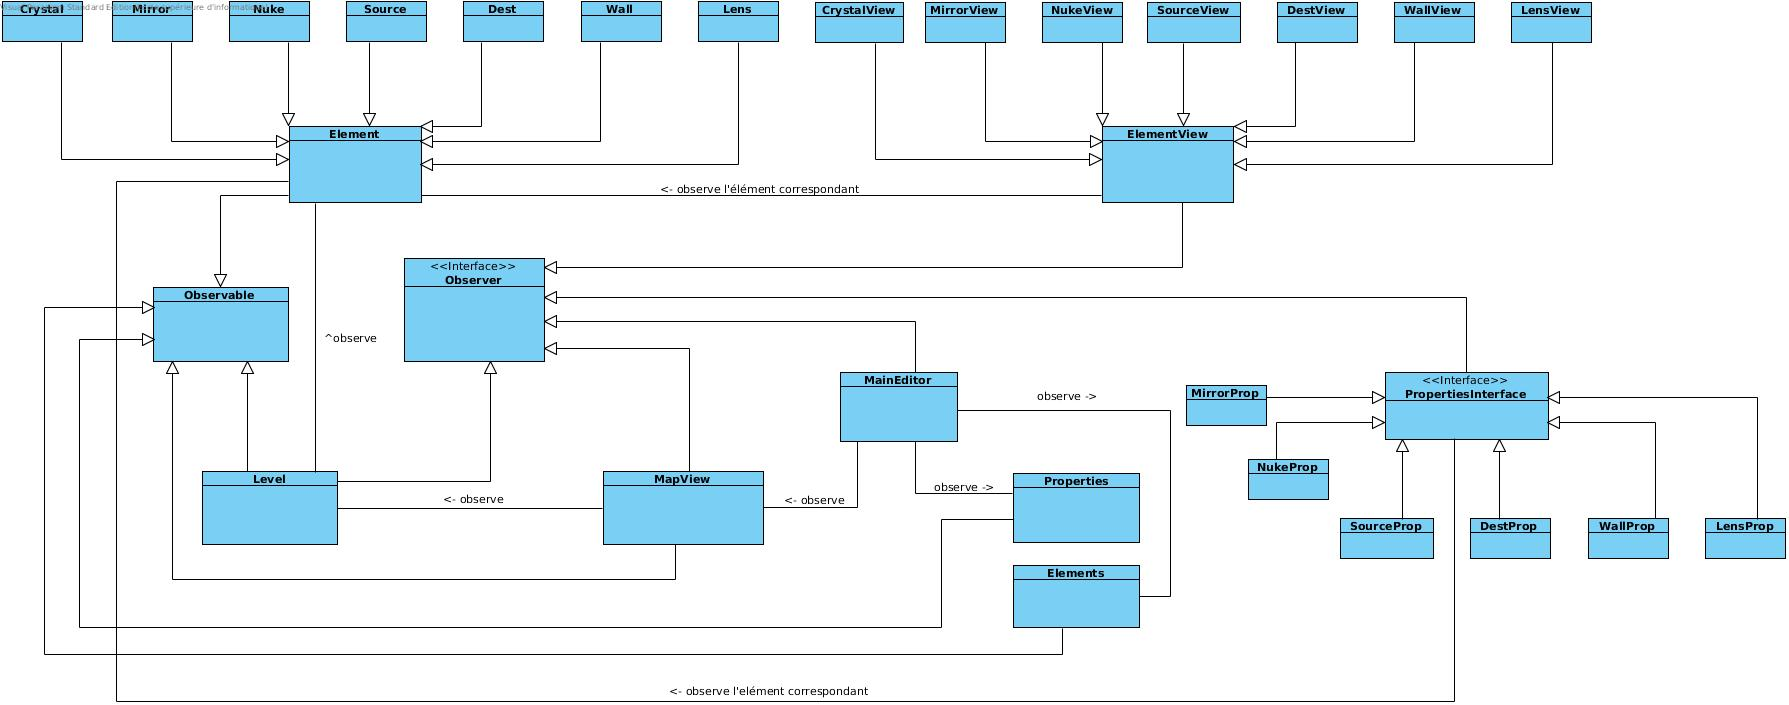
\includegraphics[scale=0.4]{Obs.jpg}
\caption{Image réalisée avec \href{http://www.visual-paradigm.com/}{Visual
	Paradigm}}
\end{figure}


\end{document}
